\documentclass[10pt]{article}



\usepackage{fancyhdr} % Required for custom headers

\usepackage{lastpage} % Required to determine the last page for the footer

\usepackage{extramarks} % Required for headers and footers

\usepackage{graphicx} % Required to insert images

\usepackage{lipsum} % Used for inserting dummy 'Lorem ipsum' text into the template

\usepackage{setspace} % Line spacing

\usepackage[title]{appendix}

\usepackage{indentfirst}

\usepackage{helvet}

\usepackage{varioref}

\usepackage{hyperref}

\usepackage{cleveref}

\usepackage[final]{pdfpages}
\renewcommand{\familydefault}{\sfdefault}

\usepackage{titlesec}

%----------------------------------------------------------------------------------------

%	SUBSUBSUBSECTION

%----------------------------------------------------------------------------------------

\titleclass{\subsubsubsection}{straight}[\subsection]

\newcounter{subsubsubsection}[subsubsection]
\renewcommand\thesubsubsubsection{\thesubsubsection.\arabic{subsubsubsection}}
\renewcommand\theparagraph{\thesubsubsubsection.\arabic{paragraph}} % optional; useful if paragraphs are to be numbered

\titleformat{\subsubsubsection}
{\normalfont\normalsize\bfseries}{\thesubsubsubsection}{1em}{}
\titlespacing*{\subsubsubsection}
{0pt}{3.25ex plus 1ex minus .2ex}{1.5ex plus .2ex}

\makeatletter
\renewcommand\paragraph{\@startsection{paragraph}{5}{\z@}%
	{3.25ex \@plus1ex \@minus.2ex}%
	{-1em}%
	{\normalfont\normalsize\bfseries}}
\renewcommand\subparagraph{\@startsection{subparagraph}{6}{\parindent}%
	{3.25ex \@plus1ex \@minus .2ex}%
	{-1em}%
	{\normalfont\normalsize\bfseries}}
\def\toclevel@subsubsubsection{4}
\def\toclevel@paragraph{5}
\def\toclevel@paragraph{6}
\def\l@subsubsubsection{\@dottedtocline{4}{7em}{4em}}
\def\l@paragraph{\@dottedtocline{5}{10em}{5em}}
\def\l@subparagraph{\@dottedtocline{6}{14em}{6em}}
\makeatother

\setcounter{secnumdepth}{4}
\setcounter{tocdepth}{4}

% Margins

\setlength\parindent{24pt}

\topmargin=-0.45in

\evensidemargin=-.25in

\oddsidemargin=-.25in

\textwidth=7.0in

\textheight=9.0in

\headsep=0.25in 



\onehalfspacing

\newcommand{\quotes}[1]{``#1''}



% Set up the header and footer

\pagestyle{fancy}

\lhead{\firstxmark} % Top right header

\chead{\projecttitle} % Top left header

\rhead{\lastxmark} % Top right header

\lfoot{\firstxmark} % Bottom left footer

\rfoot{Page\ \thepage\ of\ \pageref{LastPage}} % Bottom right footer

\renewcommand\headrulewidth{0.4pt} % Size of the header rule

\renewcommand\footrulewidth{0.4pt} % Size of the footer rule



\setlength\parindent{0pt} % Removes all indentation from paragraphs

   

%----------------------------------------------------------------------------------------

%	NAME AND CLASS SECTION

%----------------------------------------------------------------------------------------



\newcommand{\projecttitle}{Vendor Management System} % Project Title

\newcommand{\hmwkAuthorName}{Yuchen Tian, Paul Nguyen, Michael Tran} % Your name



%----------------------------------------------------------------------------------------

%	TITLE PAGE

%----------------------------------------------------------------------------------------



\title{
\vspace{2in}
\textmd{\textbf{\projecttitle} \\}
\vspace{5in}
}



\author{\textbf{\hmwkAuthorName}}

\date{} % Insert date here if you want it to appear below your name



%----------------------------------------------------------------------------------------



\begin{document}



\maketitle



%----------------------------------------------------------------------------------------

%	TABLE OF CONTENTS

%----------------------------------------------------------------------------------------



\newpage

\tableofcontents

\newpage



%----------------------------------------------------------------------------------------

%	Intro

%----------------------------------------------------------------------------------------



%----------------------------------------------------------------------------------------

%	Intro

%----------------------------------------------------------------------------------------



\section{Introduction}

\subsection{Purpose}

Internal Documentation for our senior capstone project for VCU Fall 2017. 



\subsection{Intended Audience}

Developers and Bravium Consulting Inc.

\subsection{Additional Information}

Collapse CS301 - Bravium Consulting - Vendor Management

\subsection{Contact Information}

\begin{itemize}
	\item\href{tranml3@mymail.vcu.edu}{Michael Tran}: Student Capstone 
	\item\href{tiany4@mymail.vcu.edu}{Yuchen Tian}: Student Capstone 
	\item\href{nguyenp22@mymail.vcu.edu}{Paul Nguyen}: Student Capstone 
	\item\href{dahlbergra@mymail.vcu.edu}{Robert Dahlberg}: Faculty Advisor
	\item\href{nskirpan@braviumconsulting.com}{Skirpan, Nic}: Bravium Main Contact 1
	\item\href{rnuessle@braviumconsulting.com}{Nuessle, Ryan}: Bravium Main Contact 2
	\item\href{mhade@braviumconsulting.com}{Hade, Michael}: Bravium Lead Developer
	\item\href{cnuessle@braviumconsulting.com}{Nuessle, Christine}: Bravium CEO

\end{itemize}

\subsection{Resource References}

\begin{itemize}
	\item \url{https://www.sam.gov/portal/SAM/##11}
	\item \url{https://www.naics.com/naics-drilldown-table/}
\end{itemize}



%----------------------------------------------------------------------------------------

%	Description

%----------------------------------------------------------------------------------------



\section{Overall Description}

\subsection{Product perspective}

Modernizing Vendor Management Across the Enterprise

\subsection{Product functions}

Organizations lack a streamlined process for managing external vendors, which leads to duplicative work performed on the vendor side but also within the organizations themselves. Organizations oftentimes manage vendors using disparate systems that lack work flow automation and reporting/analytics to facilitate a more efficient and accurate vendor management process.\\

There are three aspects for vendor management.
\begin{enumerate}
	
		\item Vendor acquisition: A company or organization needs to have a simple method for vendors to register themselves. The easier the process is, the more willing a vendor will be. There should be a unified form for vendors to complete. The form should envelope all aspects regarding the vendor. The details of the form are included in the data dictionary.
		\item Job selection: Currently, there is no standard for vendors to apply to job postings. For example, there are a different number of requirements for government vs private contracts such as NAICs codes, company information. 
		\item Organization: Currently there is no convenient way to organize current and past vendors/contracts. The plugin will include a role based system for each entity involved. (ex: Vendor, Vendor Manager, Business). The vendor manager will organize the entire contract/vendor acquisition process. 
\end{enumerate}



\subsection{Business requirements}

The system should work out-of-the-box for a variety of organizations, such as private companies and governmental agencies. 
A convenient, easy to access tool that makes vendor management/ contract negotiation process streamlined and simple. The tool will include workflow automation, analytics, vendor self-organization, and contract vehicles. 


\subsection{User Stories}

\subsubsection{Vendor Manager User Stories}

\begin{enumerate}
	
\item	As a Vendor Manager, I want to access ServiceNow, so that I can manage Vendors
\item	As a Vendor Manager, I want to see all job contracts, so that I can manage Vendors accordingly 
\item	As a Vendor Manager, I want to see all available Vendors, so that I can contact eligible Vendors about a new job
\item	As a Vendor Manager, I want to see all employed Vendors, so that I can manage Vendors accordingly
\item	As a Vendor Manager, I want to view a detail page on each Vendors, so that I can gather more information on the Vendor
\item	As a Vendor Manager, I want to approve each Vendors, so that I can employ them for job contracts
\item	As a Vendor Manager, I want to receive notifications from the business, so that I am up to date on current job posting
\item	As a Vendor Manager, I want to review job postings, so that I can provide feedback to the business
\item	As a Vendor Manager, I want to review job submissions, so that I can provide feedback to the business
\item	As a Vendor Manager, I want to review vendors submissions, so that I can investigate the Vendor
\item	As a Vendor Manager, I want to notify applied Vendors, so that I can provide feedback to the Vendor on the application status
\item	As a Vendor Manager, I want to notify working Vendors, so that I can gather information on the current status
\item	As a Vendor Manager, I want to see a log of status update from the Vendor, so that I can see how much of the contract is finished
\item	As a Vendor Manager, I want to set-up dates, so that I can organize meetings with Vendors
\item	As a Vendor Manager, I want to view previous contracts, so that I can keep a log of job contracts
\item	As a Vendor Manager, I want to see contracts tied with Vendors, so that I can recontact each Vendors
\item	As a Vendor Manager, I want to see a detail page on jobs contracts, so that I can adjust the work schedule to meet the deadline 
	
\end{enumerate}
	
\subsubsection{Vendor User Stories}

\begin{enumerate}
\item As a vendor, I would like to be able to access the Vendor management portal through ServiceNow, so that I can access the tool easily. 
\item As a vendor, I want to create a profile, so that I can save my company’s information and work with a business. (expand upon this)
\item As a vendor, I want to log in to my profile, so that I can quickly use the tool.
\item As a vendor, I want to be able to edit my profile, so that if anything changes within my company, it will be reflected in the vendor management tool
\item As a vendor, I want to be notified of deadlines for updating my vendor information, so that I can have accurate information in the system.
\item As a vendor, I want to be able to see jobs related to my field, so that I don’t see unnecessary information.
\item As a vendor, I want to be able to apply to jobs, so that I can start discussing details with the business 
\item As a vendor, I want to ask questions about a job I am interested in, so that I can better understand the details about the job
\item As a vendor I want to view messages sent to me over ServiceNow, so that I can respond accordingly to the messages.
\item As a vendor, I want to view my profile submission status, so that I can track the vendor approval process
\item As a vendor, I want to be notified of any important notices, so that I can respond accordingly
\item As a vendor I want to place a bid, so that the Business can view my bid and compare it to other bids
\item As a vendor, I want to add NAICS codes for my company, so that businesses can view what I am specialized in.
\item As a vendor I want to add a specialization, so that I can add a trait if it is not listed currently
\item As a vendor I want to contact the business about a job I am currently on, so that we can have a trackable communication (maybe)
\item As a vendor I want to view information about the business, so that I can see more details about that business
\item As a vendor, I want to add my company’s values, so that I can emphasize what my company stands for
\item As a vendor, I want to filter jobs based on my search results, so that I can narrow down jobs I am interested in.
\item As a vendor, I want to see a list of past jobs I have worked on, so that I can easily contact those business if I am interested in doing another job for them.

\end{enumerate}


\subsubsection{Businesses User Stories}

\begin{enumerate}
\item	As a business, I want to have a standard job form to fill out, so that I can quickly create new job postings.
\item	As a business, I want to receive notification when a vendor applies for a job, so that I can review their application.
\item	As a business, I want to receive notification when a vendor requests more information, so that I can provide the information needed.
\item	As a business, I want to edit the job posting, so that all potential vendors can view the additional information.
\item	As a business, I want to see the list of all vendors who applied for a job listing, so that I can get an overview of the downselect process.
\item	As a business, I want to send and receive SLAs, so that I can have a streamlined job application process.
\item	As a business, I want to automatically notify a vendor that they are disqualified for the job posting, so that they won’t waste time waiting for responses.
\item	As a business, I want to set the starting bid/budget, so the vendors have a guideline to work with.
\item	As a business, I want to see a list of all current bids for a job listing, so that I can have an overview of the bidding process.
\item	As a business, I want to select a vendor to be awarded the contract, so that they can work with me for the job listing.
\item	As a business, I want to upload documents attached to the job posting, so that I can provide more information that are not conveyed by the generic job form.
\item	As a business, I want to create contract vehicles, so that it is easier to work with certain governmental agencies in the future.
\item	As a business, I want to see the job history for a specific vendor, so that I know whether to work with this vendor in the future.
\item	As a business, I want to schedule online or in-person meetings with vendors, so that we can better discuss job details.
\item	As a business, I want to fill out a vendor performance form, so that I can hold vendors accountable.
\item	As a business, I want to fill out a vendor complaint form, so that I can resolve any outstanding issues.
	
\end{enumerate}

\subsection{Operating environment}
As ServiceNow is built to be an all-in-one business solution, it does not rely on third-party applications. 
ServiceNow development Is largely based on the built-in GUI based tools such as business rules, client scripts, macros, etc. For more involved tasks, JavaScript is used alongside with Glide Stack, a Web 2.0 development platform written in Java that facilitates development of forms-based workflow applications. The backend database is MySQL.

The application is made in ServiceNow as a plug. The following are the tools being used;
Framework:
\begin{itemize}
	\item ServiceNow \url{https://braviumdemo1.service-now.com/navpage.do}
	\item Angular \url{https://medium.baqend.com/angular-2-by-example-e85a09fa6480}
\end{itemize}
Language:
\begin{itemize}
	\item Java
	\item Html
	\item JS \url{https://javascript.info/}
\end{itemize}


\subsection{User environment}

ServiceNow, the user would enable the plug-in then input all vendor information. Unless needed the user can update the vendor information. Can also import data from other tables. 

\subsection{Stakeholders}
\begin{itemize}
	\item	Vendor: provides goods/services to the Business
	\item	Vendor Manager: oversees the vendors and their interactions with the Businesses
	\item	Business: posts jobs and seeks vendors to fulfill contracts  
	
\end{itemize}

\subsection{Constraints}
Must be built in the ServiceNow environment.

%----------------------------------------------------------------------------------------

%	System

%----------------------------------------------------------------------------------------



%----------------------------------------------------------------------------------------

%	System feature A

%----------------------------------------------------------------------------------------



\section{System Features}

\subsection{Vendor Profile}

\subsubsection{Description and priority}

Vendor Profile houses all the general vendor information. Can be customizable to the owner liking

\subsubsection{Action/result}

See Work-flow See Work-flow on the next page

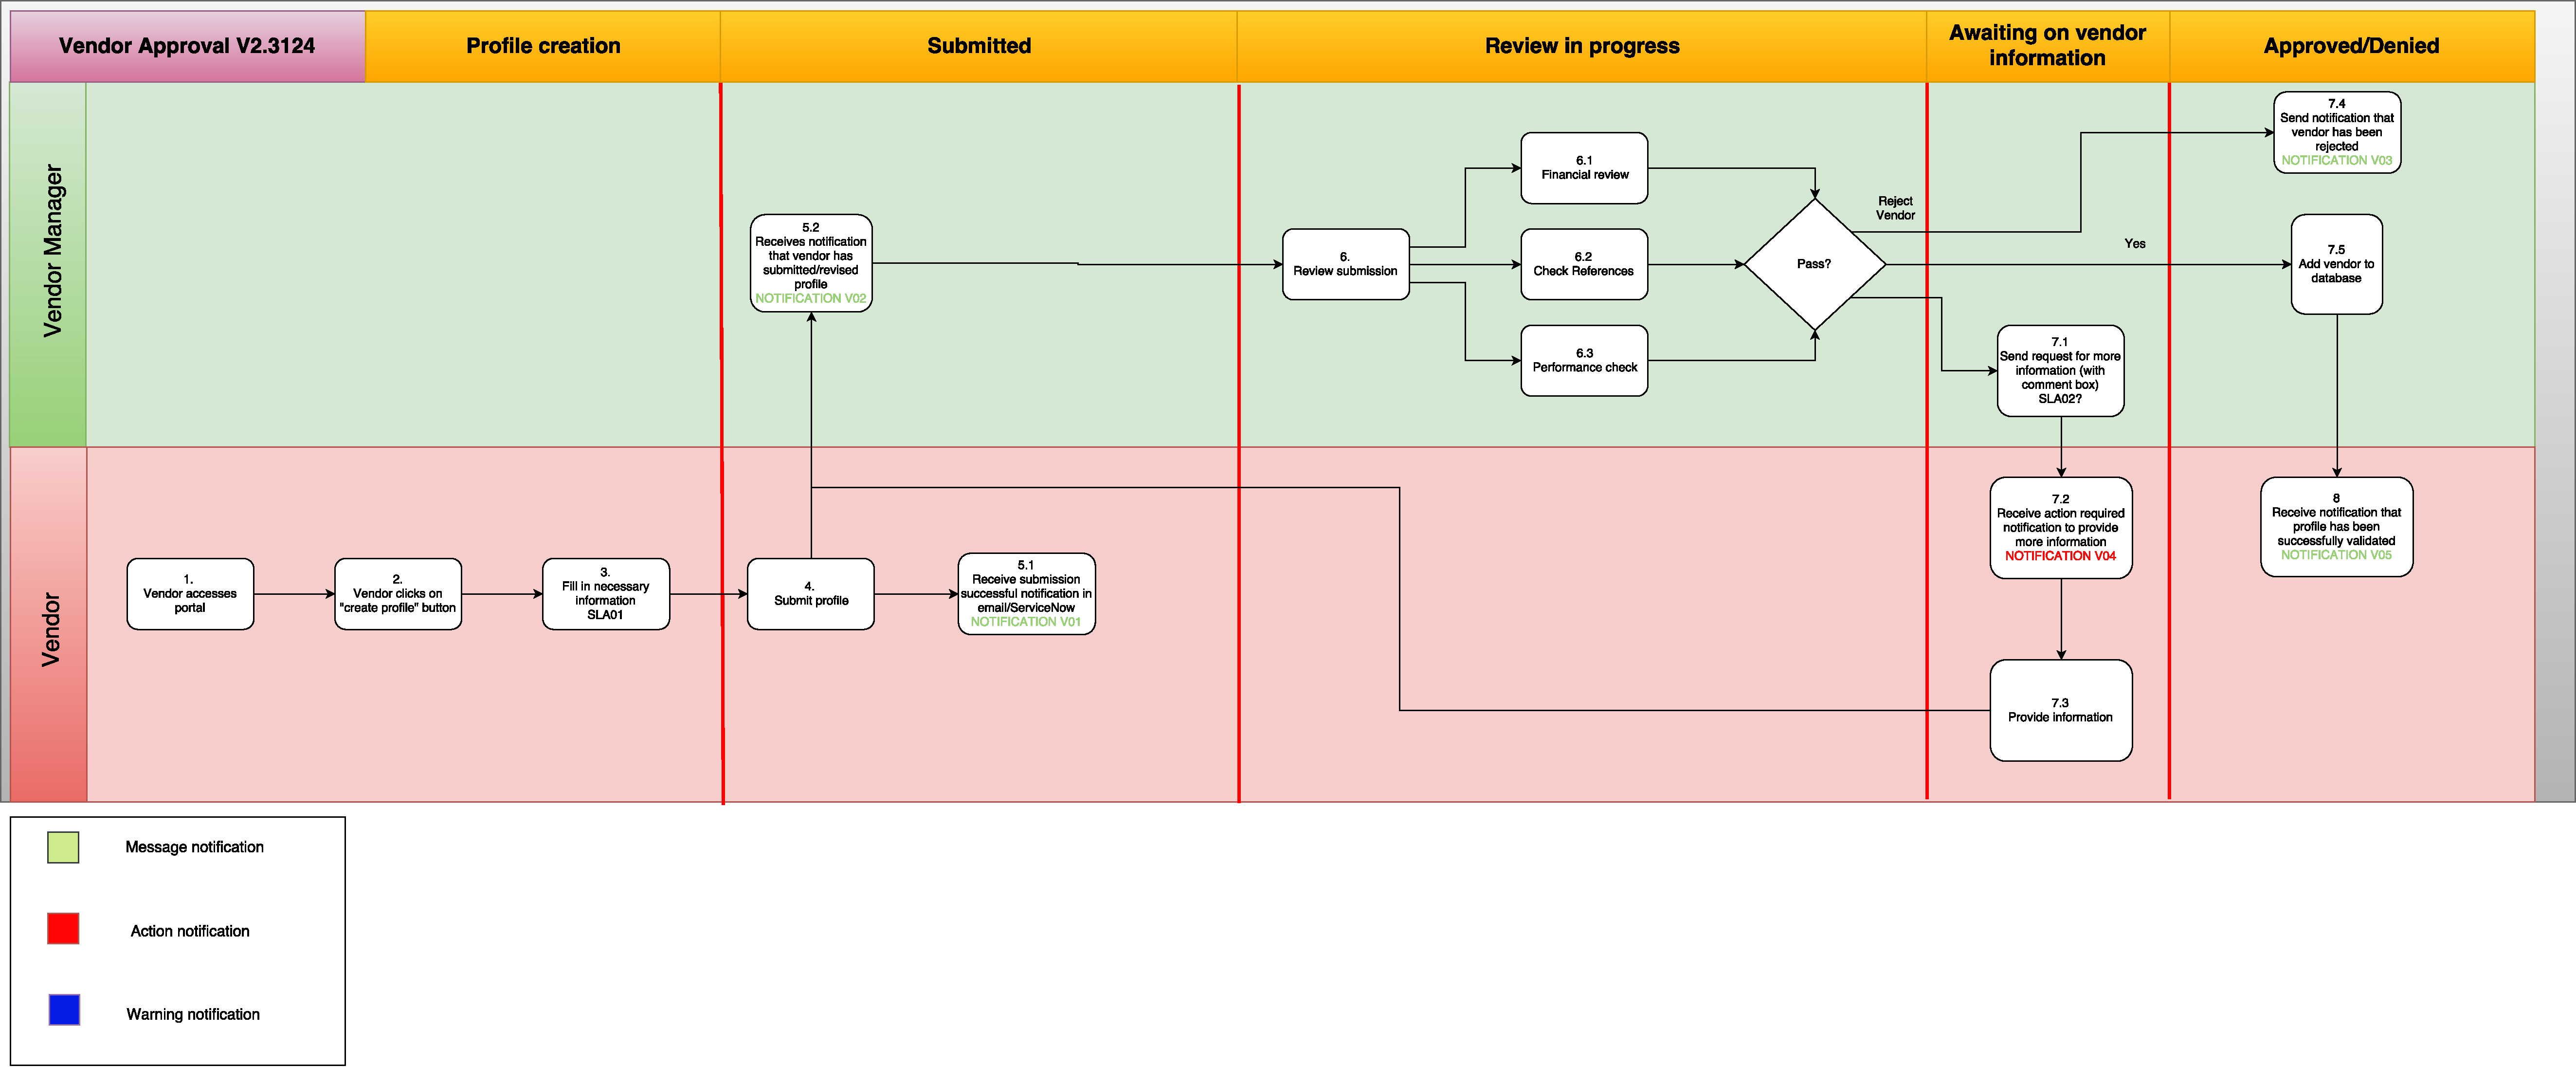
\includepdf[pages={-},angle=-90]{../Workflow/Vendor_Profile_Approval/Vendor_Profile_Approval_11_2.pdf}

\subsubsection{ Functional requirements}

\lipsum[10]

%----------------------------------------------------------------------------------------

%	System feature B

%----------------------------------------------------------------------------------------



\subsection{System feature B}

\subsubsection{Vendor Job Application}

After the vendor makes a profile now the vendor can apply to jobs from whats is available

\subsubsection{Action/result}

See Work-flow on the next page

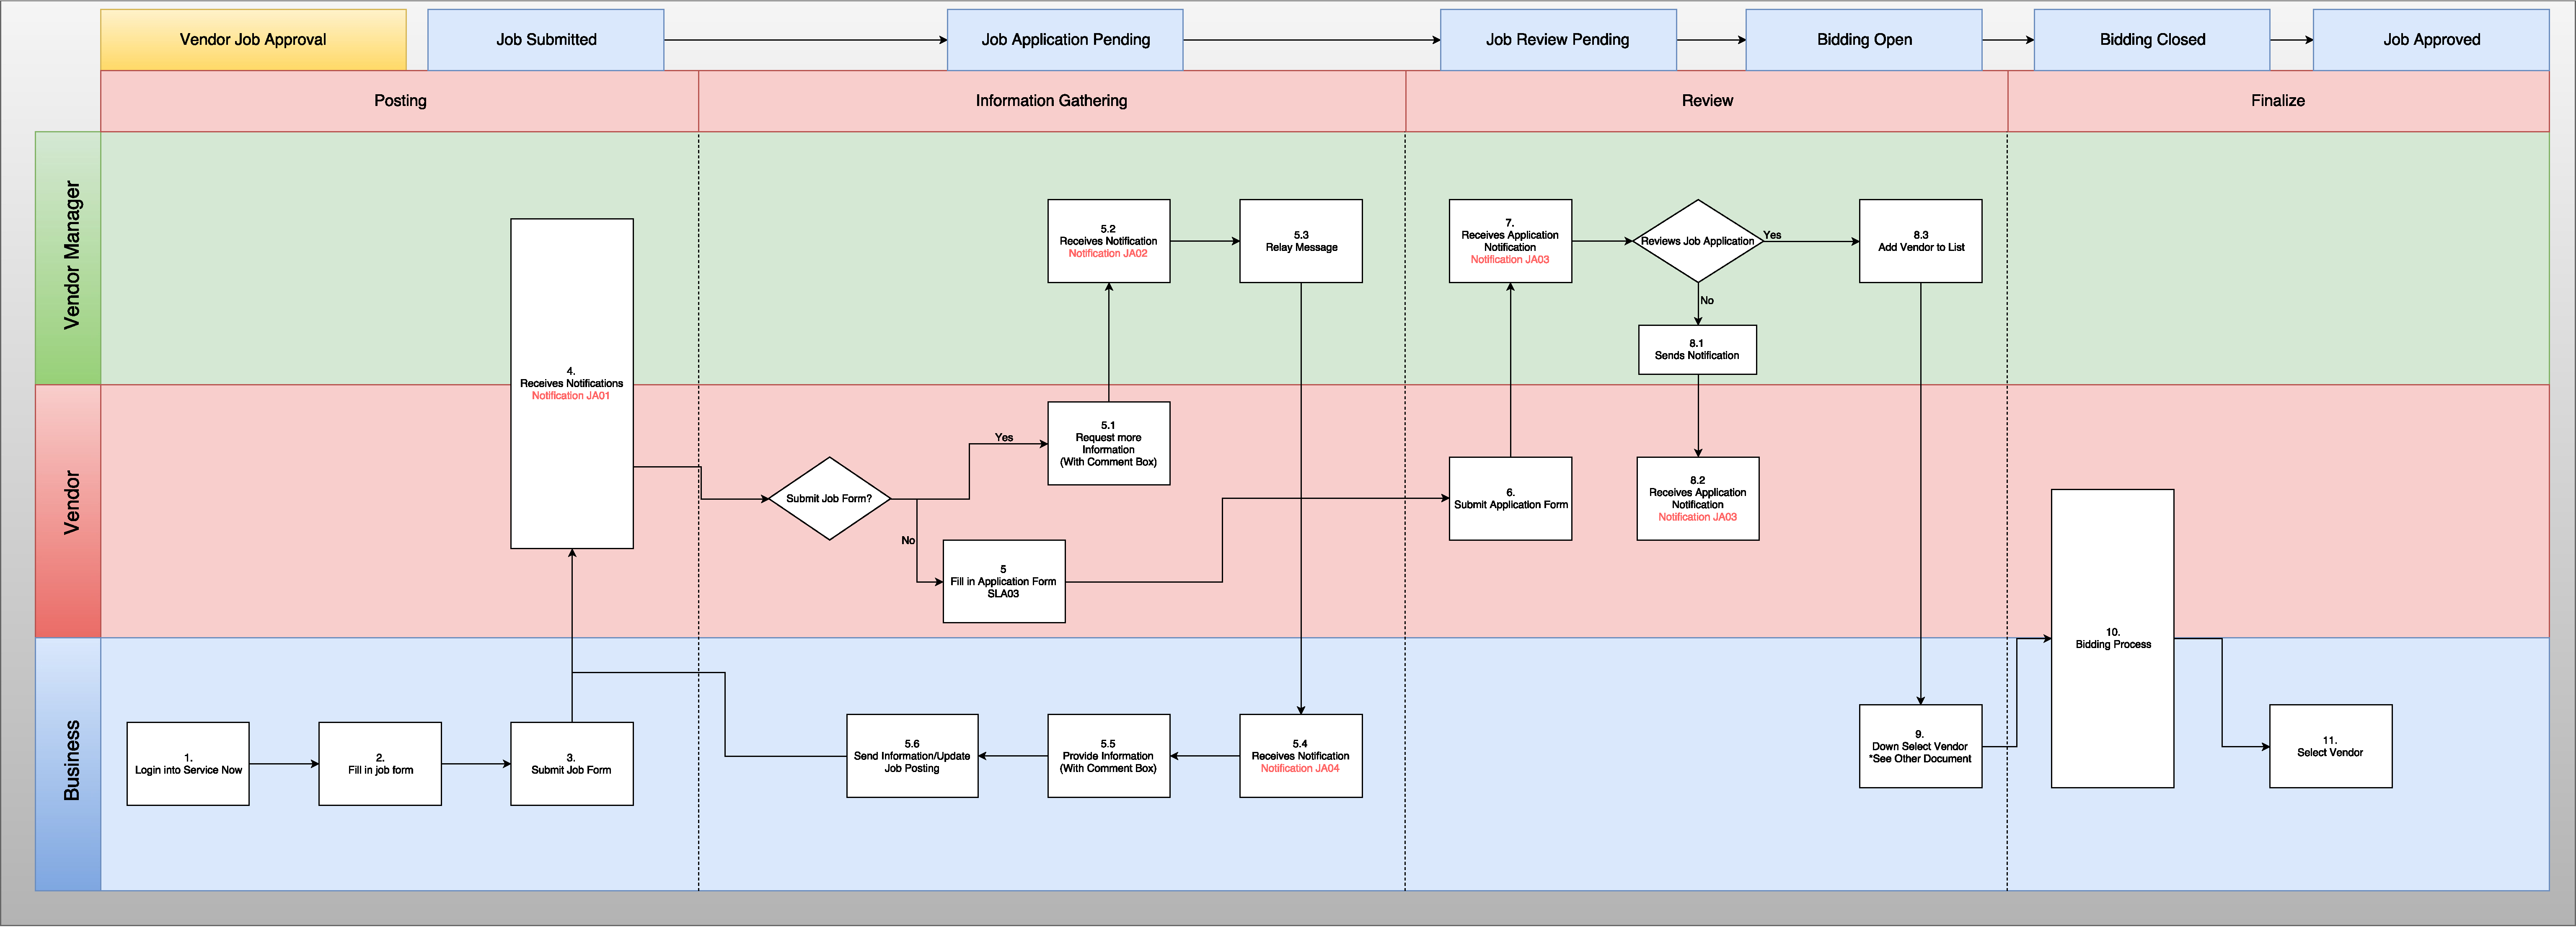
\includepdf[pages={-},angle=-90]{../Workflow/Vendor_Job_Application/Vendor_Job_Application_11_2.pdf}

\subsubsection{ Functional requirements}

\lipsum[10]








\end{document}
